% uklad dokumentu
	\documentclass{article}
	\usepackage{xparse}
	\usepackage[margin=1.5cm]{geometry}
    \usepackage{enumerate} 
	\frenchspacing
    \linespread{1.0}
    \setlength{\parindent}{0pt}

% jezyk polski
	\usepackage[T1]{fontenc}
	\usepackage[polish]{babel}
	\usepackage[utf8]{inputenc}
 
% pakiety matematyczne
    \let\lll\undefined
    \usepackage{mathtools}
	\usepackage{amssymb}
    \usepackage{amsthm}
	\usepackage{amsmath}
	\usepackage{amsfonts}
	\usepackage{tikz}

	\usepackage{float}	
	
% pakiety do automatów
	\usetikzlibrary{automata, arrows.meta, positioning, arrows}
	
% wykresiki
	\usepackage{pgfplots}
	\pgfplotsset{compat = newest}
	\usepackage{graphicx}
	\usepackage{subcaption}

    \title{\textbf{Algorytmy Metaheurystyczne\\Komiwojażer Heurystycznie}}
    \author{Gabriel Budziński(254609)\\Franciszek Stepek (256310)}
    \date{}
    
    
\begin{document} 
\maketitle

\section*{Przedmowa}
Na samym początku omówimy po krótce użyte algorytmy, oraz zastanowimy się nad ich złożonością obliczeniową, natomiast dalej dopiero przejdziemy do opisu eksperymentów.

\section{Podsumowanie złożoności obliczeniowych implementacji}
\subsection{K-Random}
Algorytm polega na losowaniu kolejności odwiedzania wierzchołków. Każde z wylosowanych rozwiązań jest porównywane z poprzednim najlepszym. W naszej implementacji losowanie rozwiązania odbywało się w czasie liniowym. W takim samym czasie obliczana jest również funkcja celu. Dla $k$ prób złożoność jest w takim razie rzędu $O(k\cdot n\cdot n) = O(k \cdot n^2)$.

\subsection{Nearest Neighbor}
Algorytm polega na zachłannym szukaniu ścieżki rozpoczynając od zadanego wierzchołka i przechodząc do najbliższego jeszcze nie odwiedzonego. Złożoność jest rzędu $O(n^2)$, ponieważ w każdym wierzchołku musimy przeszukać zbiór pozostałych, aby znaleźć najbliższy. Chcąc uzyskać lepsze wyniki, możemy zainicjować algorytm we wszystkich wierzchołkach i wybrać najlepszą trasę. Przy takiej modyfikacji złożoność zwiększa się do $O(n^2 \cdot n + n\cdot n) = O(n^3)$, ponieważ pierwotny algorytm wykonujemy $n$ razy i $n$-krotnie musimy obliczyć wartość funkcji celu.

\subsection{Nearest Branching Neighbor}
Algorytm jest modyfikacją powyższego algorytmu, która rozstrzyga, który wierzchołek obrać jako następny w przypadku równej odległości do nich. Złożoność jest bardzo zależna od stryktury problemu i głębokości zagłębiania przeszukiwań. Zakładając, że problem ma strukturę drzewa, gdzie wierzchołek ma dwa równo odległe od siebie następniki, każdy poziom przeszukiwań ma wzrost wykładniczy.

\subsection{2-Opt}
Algorytm polega na wybieraniu kawałka istniejącej już trasy, a następnie wstawienie go z powrotem, ale w odwrotnej kolejności. Czynność tę powtarzamy, aż nie będziemy już uzyskiwać zysku długości trasy. Złożoność algorytmu można ulepszyć nie wyliczając za każdym odwróceniem funkcji celu, a jedynie odejmować i dodawać wartości dwóch usuniętych i dwóch dodanych krawędzi $O(4)$ $\approx$ \textit{negl.}. Złożoność obliczeniowa w naszej implementacji jest rzędu $O(n^2\cdot n) = O(n^3)$, ponieważ operacja zmiany kolejności kawałka trasy jest $O(n)$.

\subsection{3-Opt}
Algorytm jest analogiczny do powyższego, z tą różnicą, że teraz dzielimy trasę na trzy, a nie na dwa kawałki. Co za tym idzie, to także zwiększa nam złożoność obliczeniową, ponieważ przecchodzimy przez wszystkie trójki krawędzi. Zatem mamy tutaj łącznie rząd $O(n^3\cdot n) = O(n^4)$ (operacja sprawdzenia każdego przypadku jest co prawda większa, ale w dalszym ciągu $O(1)$, a zamiana kawałka trasy w tym samym czasie co powyżej).

\section{Opis eksperymentów}
\subsection{Implementacja}
Algorytmy implementujemy w języku \texttt{C/C++}, odległości między wierzchołkami są przechowywane jako pełne tablice dwuwymiarowe typu \texttt{int}, a trasy są w kontenerach \texttt{vector}, co ułatwia operacje odwracania i mieszania.\\
Korzystaliśmy z kompilatora g++ wraz z użyciem flag -lSDL2 (używanej przy wizualizacji, wraz z odpowiednim dla danego systemu operacyjnego podlinkowania do folderu zawierającego) oraz -lpthread (przy korzystaniu z wielowątkowości)

\subsection{Sprzęt}
Programy były testowane na dwóch maszynach, laptopie \textit{Lenovo} i komputerze stacjonarnym. Obie jednostki są wyposażone w procesor architektury \texttt{x86} marki \texttt{intel} oraz 16GB pamięci RAM.

\subsubsection{Pececik}
Komputer stacjonarny posiada procesor sześciordzeniowy i5-10600K 4,1 GHz (o obniżonym napięciu operacyjnym).
\subsubsection{Lapek}
Laptop posiada procesor czterordzeniowy i7-6700HQ 2,6 GHz

\subsection{Instancje}
\subsubsection{Przykłady TSPLIB}
W części eksperymentów użyto instancji euklidejskiego problemu komiwojażera.

\subsubsection{Instancje losowe}
W celu zwiększenia liczności i dokładności testów spreparowano losowo generowane instancje eukidejskiego problemu komiwojażera.

\subsection{Metodologia/cel}

Testy przeprowadzono za pomocą zaimplementowanych w tym celu funkcji ku jak największej automatyzacji. Dane o przeprowadzonych testach zapisywano do plików tekstowych w formacie CSV, a następnie poddane analizie. Testowanie miało na celu wskazanie mocnych i słabych stron zaimplementowanych heurystyk, jak i ich porównanie.

\subsection{Opis wyników}
Testy Wilcoxona dla poszczególnych algorytmów:
\begin{itemize}
	\item W pierwszej dużej tabeli będziemy mieli zestawienie 3 algorytmów
	\item W drugiej (Już nieco 'ciekawszej') Zobaczymy jak na rozwiązanie \textit{2-Opt} wpływają warunki początkowe (zarówno czasowo, jak i w kontekście funkcji Celu)
	\item W trzeciej otrzymamy większe zestawienie różnych przypadków dla wariantów \textit{Nearest Neighbor}
	\item W czwartej zobaczymy porownanie działania \textit{2-Opta} z \textit{3-Optem}, wraz z zestawieneim, ile procentowo polepszył się wynik, oraz z jakim nakładem kosztu to się stało.
\end{itemize}

\newpage
\subsubsection{Część I}
Tabela numer 1:
\begin{table}[h!]
\centering
\begin{tabular}{c||c|c|c||c|c c c|c|c} 
Nr. Instancji & 1 & 2 & 3 & 4 & 5 &  & 1-2 & 1-3 & 4-5 \\
\hline
1 & 3157 & 32621 & 2846 & 2922 & 33913 &  & -29464 & 311 & -30991 \\
2 & 8980 & 29990 & 8385 & 8746 & 25809 &  & -21010 & 595 & -17063 \\
3 & 135737 & 610252 & 126892 & 128097 & 622778 &  & -474515 & 8845 & -494681 \\
4 & 7579 & 47194 & 7098 & 6741 & 49975 &  & -39615 & 481 & -43234 \\
5 & 8191 & 53545 & 7157 & 7372 & 54720 &  & -45354 & 1034 & -47348 \\
6 & 803 & 3509 & 714 & 677 & 3560 &  & -2706 & 89 & -2883 \\
7 & 511 & 1586 & 454 & 443 & 1750 &  & -1075 & 57 & -1307 \\
8 & 642 & 2606 & 561 & 595 & 2645 &  & -1964 & 81 & -2050 \\
9 & 27807 & 168501 & 23737 & 23006 & 172442 &  & -140694 & 4070 & -149436 \\
10 & 33633 & 270344 & 28612 & 29756 & 242459 &  & -236711 & 5021 & -212703 \\
11 & 35859 & 331888 & 31749 & 34109 & 345599 &  & -296029 & 4110 & -311490 \\
12 & 29158 & 154024 & 25393 & 25014 & 174054 &  & -124866 & 3765 & -149040 \\
13 & 34499 & 256477 & 28435 & 29312 & 253834 &  & -221978 & 6064 & -224522 \\
14 & 36980 & 338421 & 33375 & 34698 & 339346 &  & -301441 & 3605 & -304648 \\
15 & 26227 & 174278 & 23107 & 22850 & 178774 &  & -148051 & 3120 & -155924 \\
16 & 26947 & 173366 & 24721 & 25011 & 174970 &  & -146419 & 2226 & -149959 \\
17 & 27460 & 170965 & 24459 & 23810 & 154305 &  & -143505 & 3001 & -130495 \\
18 & 20356 & 126612 & 18281 & 15972 & 121878 &  & -106256 & 2075 & -105906 \\
19 & 54019 & 593697 & 49141 & 46246 & 606262 &  & -539678 & 4878 & -560016 \\
20 & 54019 & 582949 & 49141 & 45758 & 575474 &  & -528930 & 4878 & -529716 \\
21 & 68964 & 1405305 & 60930 & 62216 & 1415877 &  & -1336341 & 8034 & -1353661 \\
22 & 331103 & 6434381 & 282758 & 279968 & 6392975 &  & -6103278 & 48345 & -6113007 \\
23 & 46680 & 597495 & 45340 & 49462 & 572145 &  & -550815 & 1340 & -522683 \\
24 & 69297 & 735352 & 61910 & 64640 & 677100 &  & -666055 & 7387 & -612460 \\
25 & 120769 & 842650 & 110103 & 107601 & 882692 &  & -721881 & 10666 & -775091 \\
26 & 61652 & 821860 & 61400 & 68116 & 823348 &  & -760208 & 252 & -755232 \\
27 & 85699 & 988886 & 79996 & 81923 & 1028352 &  & -903187 & 5703 & -946429 \\
28 & 94683 & 1638917 & 87542 & 88659 & 1635424 &  & -1544234 & 7141 & -1546765 \\
29 & 58023 & 1137733 & 56765 & 55439 & 1183487 &  & -1079710 & 1258 & -1128048 \\
30 & 59890 & 766136 & 52403 & 56468 & 791951 &  & -706246 & 7487 & -735483 \\
31 & 131281 & 1940053 & 118468 & 119774 & 1962350 &  & -1808772 & 12813 & -1842576 \\
32 & 153462 & 586378 & 121315 & 121297 & 568936 &  & -432916 & 32147 & -447639 \\
33 & 2752 & 22583 & 2497 & 2684 & 22420 &  & -19831 & 255 & -19736 \\
34 & 8605 & 110285 & 7566 & 7628 & 114431 &  & -101680 & 1039 & -106803 \\
35 & 11054 & 183204 & 9415 & 9627 & 182635 &  & -172150 & 1639 & -173008 \\
36 & 1554 & 8755 & 1418 & 1346 & 8903 &  & -7201 & 136 & -7557 \\
37 & 830 & 3585 & 770 & 775 & 3466 &  & -2755 & 60 & -2691 \\
38 & 152493 & 1629073 & 139697 & 140164 & 1576951 &  & -1476580 & 12796 & -1436787 \\
39 & 5030 & 41053 & 4418 & 4294 & 42391 &  & -36023 & 612 & -38097 \\
 \end{tabular}
\end{table}

Przy czym kolejne kolumny 'numeryczne' oznaczają:
\begin{itemize}
	\item 1 - Wartość funkcji Celu dla algorytmu \textit{Nearest Neighbor} startującego z wybranego 'miasta'
	\item 2 - Wartość funkcji Celu dla algorytmu \textit{K-Random} działającego tak długo, jak z kolumny 1
	\item 3 - Wartość funkcji Celu dla algorytmu \textit{2-Opt} startującego z rozwiązania w punkcie 1
	\item 4 - Wartość funkcji Celu dla algorytmu \textit{2-Opt} startującego z losowej instancji
	\item 5 - Wartość funkcji Celu dla algorytmu \textit{K-Random} działającego tak długo, jak z kolumny 4
\end{itemize}

A teraz jak rozumieć kolejne kolumny 'różnicowe':
\begin{itemize}
	\item 1-2 - Porównanie działania KR z NN dla tego samego budżetu obliczeniowego
	\item 1-3 - 'Dowód', że 2O rzeczywiście poprawia rozwiązanie startowe
	\item 4-5 - Porównanie działania KR z 2O dla tego samego budżetu obliczeniowego
\end{itemize}

Zauważmy, że we wszystkich tych kolumnach każda z wartości jest tego samego znaku, zatem bez dokładniejszej analizy można powiedzieć, że wartość statystyki testowej dla testu Wilcoxona będzie równa 0, zatem jednoznacznie powie nam, który z algorytmów zwraca zawsze lepsze rozwiązanie. Pojawia się nam zatem następująca zależność (gdzie znak '<' oznacza, że lewa wartość zwraca nam 'gorsze' rozwiązanie od prawego):
\[\textit{K-Random} < \textit{Nearest Neighbor} < \textit{2-Opt}\]

\newpage
\subsubsection{Część II}
Tabela numer 2:
\begin{table}[h!]
\centering
\begin{tabular}{c||c|c||c|c||c c c|c}
Nr. Instancji & NN & KR & NN-KR & |NN-KR| & Rangi & & NN(T) & KR(T)\\
\hline
1 & 2846 & 2992 & -146 & 146 & 11 &  & 0.115728 & 3.10199 \\
2 & 8385 & 7967 & 418 & 418 & 16 &  & 0.00120772 & 0.00922684 \\
3 & 126892 & 124006 & 2886 & 2886 & 29 &  & 0.0187193 & 0.145382 \\
4 & 7098 & 6988 & 110 & 110 & 8 &  & 0.0138299 & 0.184798 \\
5 & 7157 & 7080 & 77 & 77 & 6.5 &  & 0.0393003 & 0.338091 \\
6 & 714 & 689 & 25 & 25 & 4 &  & 0.00987954 & 0.0552343 \\
7 & 454 & 461 & -7 & 7 & 2 &  & 0.00119699 & 0.0103625 \\
8 & 561 & 567 & -6 & 6 & 1 &  & 0.00364293 & 0.0333502 \\
9 & 23737 & 24667 & -930 & 930 & 19 &  & 0.0154935 & 0.137051 \\
10 & 28612 & 29780 & -1168 & 1168 & 21 &  & 0.053393 & 0.313875 \\
11 & 31749 & 32634 & -885 & 885 & 18 &  & 0.144667 & 0.836886 \\
12 & 25393 & 24066 & 1327 & 1327 & 22 &  & 0.0138314 & 0.0914137 \\
13 & 28435 & 29226 & -791 & 791 & 17 &  & 0.037316 & 0.41158 \\
14 & 33375 & 33294 & 81 & 81 & 7 &  & 0.109228 & 0.997454 \\
15 & 23107 & 22870 & 237 & 237 & 13 &  & 0.0119046 & 0.102974 \\
16 & 24721 & 23678 & 1043 & 1043 & 20 &  & 0.01084 & 0.0888192 \\
17 & 24459 & 24275 & 184 & 184 & 12 &  & 0.0122842 & 0.114743 \\
18 & 18281 & 15962 & 2319 & 2319 & 26 &  & 0.0165922 & 0.0705111 \\
19 & 49141 & 46422 & 2719 & 2719 & 28 &  & 0.322236 & 4.21766 \\
20 & 49141 & 45633 & 3508 & 3508 & 32 &  & 0.343797 & 2.56742 \\
21 & 60930 & 61190 & -260 & 260 & 14 &  & 27.5015 & 656.948 \\
22 & 282758 & 287980 & -5222 & 5222 & 34 &  & 11.1163 & 179.428 \\
23 & 45340 & 52126 & -6786 & 6786 & 38 &  & 0.0065809 & 0.110337 \\
24 & 61910 & 67957 & -6047 & 6047 & 36 &  & 0.0144687 & 0.196237 \\
25 & 110103 & 103341 & 6762 & 6762 & 37 &  & 0.0155958 & 0.195165 \\
26 & 61400 & 66836 & -5436 & 5436 & 35 &  & 0.00640445 & 0.246059 \\
27 & 79996 & 82941 & -2945 & 2945 & 30 &  & 0.0186396 & 0.358017 \\
28 & 87542 & 90788 & -3246 & 3246 & 31 &  & 0.062336 & 0.966489 \\
29 & 56765 & 58313 & -1548 & 1548 & 24 &  & 0.0857857 & 2.09062 \\
30 & 52403 & 56508 & -4105 & 4105 & 33 &  & 0.221278 & 4.1955 \\
31 & 118468 & 119808 & -1340 & 1340 & 23 &  & 0.673865 & 13.1858 \\
32 & 121315 & 118891 & 2424 & 2424 & 27 &  & 0.00617383 & 0.0256009 \\
33 & 2497 & 2624 & -127 & 127 & 10 &  & 0.046445 & 0.83168 \\
34 & 7566 & 7643 & -77 & 77 & 6.5 &  & 1.95213 & 32.5976 \\
35 & 9415 & 9687 & -272 & 272 & 15 &  & 4.56492 & 81.1747 \\
36 & 1418 & 1399 & 19 & 19 & 3 &  & 0.0119262 & 0.103982 \\
37 & 770 & 799 & -29 & 29 & 5 &  & 0.00323845 & 0.0298058 \\
38 & 139697 & 137507 & 2190 & 2190 & 25 &  & 0.0786318 & 0.723296 \\
39 & 4418 & 4531 & -113 & 113 & 9 &  & 0.0935837 & 1.57451 \\
\end{tabular}
\end{table}

Przy czym kolejne kolumny oznaczają:
\begin{itemize}
	\item NN - Wartość funkcji Celu dla algorytmu \textit{2-Opt} startującego z rozwiązania znalezionego przez algorytm \textit{Nearest Neighbor}
	\item KR - Wartość funkcji Celu dla algorytmu \textit{2-Opt} startującego z rozwiązania znalezionego przez algorytm \textit{K-Random} (Startowe rozwiązanie w tym samym czasie, co startowe dla NN)
	\item Kolejne 2  kolumny znaczą dokładnie to, co ich nazwa, natomist ostatnia wyznacza rangi dla testu Wilcoxona
\end{itemize}

A teraz policzmy jeszcze tylko 2 sumy dla Wilcoxona:
\begin{itemize}
	\item $T_+ = 315.5$
	\item $T_- = 432.5$
\end{itemize}
Zatem nasza statystyka końcowa będzie wynosiła $315.5$. No jest to dosyć dużo, a fakt, że wynosi ona około 1/2 sumy obu statystyk sugeruje, że w istocie obie metody działają 'bardzo podobnie'\\

Prawa strona tabeli jest analogiczna do lewej, ale tym razem zamiast wartości Celu mamy czas działania samej części \textit{2-Opt}.\\
Jak widać, czas działania przy starcie z \textit{K-Randoma} jest znacznie dłuższy, ale (w połączeniu z danymi otrzymanymi w tabeli 1) można powiedzieć, że łatwo uzależnić czas działania algorytmu 2-Opt od pierwotnego rozwiązania - jeżeli jest znacznie 'lepsze', to także widać, że różnice w czasie są znacznie wyższe (później zobaczymy, że przy względnie niewielkich różnicach warunków początkowych ta zależność znika).\\

\newpage
\subsubsection{Część III}
Tabela numer 3:
\begin{table}[h!]
\centering
\begin{tabular}{c||c|c|c|c c c|c|c|c}
Nr.In & 1N & FN & 1B & FB &  & 1N(T) & FN(T) & 1B(T) & FB(T) \\
\hline
1 & 3157 & 2975 & 3452 & 2998 &  & 0.000644468 & 0.0983119 & 0.0048885 & 1.01056 \\
2 & 8980 & 8181 & 8980 & 8181 &  & 2.07E-05 & 0.00103294 & 3.76E-05 & 0.00205635 \\
3 & 135737 & 133953 & 129421 & 128279 &  & 0.000146889 & 0.0121529 & 0.000282864 & 0.0361393 \\
4 & 7579 & 7129 & 7198 & 6908 &  & 0.000104299 & 0.0139546 & 0.000241166 & 0.0310817 \\
5 & 8191 & 7113 & 8191 & 7113 &  & 0.000134752 & 0.0224471 & 0.000239433 & 0.0382092 \\
6 & 803 & 746 & 804 & 748 &  & 6.75E-05 & 0.00723383 & 0.000454636 & 0.0460773 \\
7 & 511 & 482 & 545 & 499 &  & 2.06E-05 & 0.00110371 & 0.000153318 & 0.00747459 \\
8 & 642 & 608 & 621 & 599 &  & 6.48E-05 & 0.0034514 & 0.000231878 & 0.0173178 \\
9 & 27807 & 24698 & 26854 & 24815 &  & 6.99E-05 & 0.00736386 & 0.00012696 & 0.0131532 \\
10 & 33633 & 31479 & 33612 & 31479 &  & 0.000222951 & 0.0240762 & 0.00021405 & 0.0365781 \\
11 & 35859 & 34543 & 35794 & 34543 &  & 0.000252144 & 0.0555201 & 0.000354758 & 0.0790306 \\
12 & 29158 & 25884 & 29158 & 25884 &  & 9.39E-05 & 0.00853953 & 0.000109656 & 0.0112842 \\
13 & 34499 & 31611 & 32825 & 31611 &  & 0.000131333 & 0.0222619 & 0.000253897 & 0.0373115 \\
14 & 36980 & 35389 & 36980 & 35389 &  & 0.000236748 & 0.0511064 & 0.000379147 & 0.0778277 \\
15 & 26227 & 23660 & 26227 & 23564 &  & 6.77E-05 & 0.00713671 & 0.000131215 & 0.0138976 \\
16 & 26947 & 24852 & 26947 & 24852 &  & 0.000125232 & 0.00788403 & 0.000222792 & 0.0115013 \\
17 & 27460 & 24782 & 27460 & 24782 &  & 6.63E-05 & 0.00694331 & 0.000201731 & 0.0129614 \\
18 & 20356 & 16935 & 20356 & 16935 &  & 5.77E-05 & 0.00701994 & 0.000113084 & 0.0166362 \\
19 & 54019 & 49201 & 54019 & 49201 &  & 0.000421003 & 0.166132 & 0.000678634 & 0.260951 \\
20 & 54019 & 49201 & 54019 & 49201 &  & 0.000420879 & 0.155087 & 0.000638746 & 0.240323 \\
21 & 68964 & 68531 & 70315 & 67864 &  & 0.0102591 & 14.3142 & 0.0157081 & 24.5947 \\
22 & 331103 & 313745 & 322807 & 310967 &  & 0.0042375 & 4.41593 & 0.0108562 & 11.6176 \\
23 & 46680 & 46680 & 49166 & 47899 &  & 5.57E-05 & 0.00624229 & 0.000471479 & 0.0663509 \\
24 & 69297 & 67055 & 71550 & 67323 &  & 8.92E-05 & 0.00915955 & 0.000177797 & 0.0226451 \\
25 & 120769 & 114553 & 120769 & 114553 &  & 8.82E-05 & 0.012921 & 0.000207303 & 0.0303293 \\
26 & 61652 & 60964 & 61652 & 60964 &  & 9.07E-05 & 0.0139036 & 0.000168004 & 0.0304266 \\
27 & 85699 & 79564 & 85699 & 79564 &  & 0.000102496 & 0.0173458 & 0.000168221 & 0.0335902 \\
28 & 94683 & 92552 & 94683 & 92903 &  & 0.000204923 & 0.0498144 & 0.00163079 & 0.352259 \\
29 & 58023 & 54491 & 58635 & 54604 &  & 0.000284032 & 0.0803066 & 0.000632295 & 0.193229 \\
30 & 59890 & 58279 & 58151 & 58151 &  & 0.000401408 & 0.125099 & 0.00113758 & 0.380743 \\
31 & 131281 & 127230 & 131445 & 126062 &  & 0.000791101 & 0.383126 & 0.0016203 & 0.873932 \\
32 & 153462 & 130921 & 153462 & 130921 &  & 3.31E-05 & 0.00248934 & 6.17E-05 & 0.00508362 \\
33 & 2752 & 2612 & 2632 & 2606 &  & 0.000155953 & 0.0351781 & 0.000429553 & 0.113054 \\
34 & 8605 & 7993 & 8700 & 7934 &  & 0.00137766 & 0.857353 & 0.0040416 & 2.48614 \\
35 & 11054 & 10540 & 10763 & 10657 &  & 0.00274642 & 2.70393 & 0.00916338 & 7.70218 \\
36 & 1554 & 1437 & 1544 & 1432 &  & 5.00E-05 & 0.00510014 & 0.000238881 & 0.022591 \\
37 & 830 & 796 & 801 & 751 &  & 7.09E-05 & 0.00241989 & 0.000155393 & 0.0108239 \\
38 & 152493 & 140486 & 152493 & 140486 &  & 0.000206588 & 0.049608 & 0.00139074 & 0.239691 \\
39 & 5030 & 4578 & 4941 & 4691 &  & 0.000318213 & 0.0560495 & 0.000668361 & 0.163452 \\
\end{tabular}
\end{table}

Przy czym kolejne kolumny oznaczają:
\begin{itemize}
	\item 1N - Wartość funkcji Celu dla algorytmu \textit{Nearest Neighbor} startującego z wybranego miasta
	\item FN - Wartość funkcji Celu dla algorytmu \textit{Nearest Neighbor} startującego z każdego miasta, i wybierający najlepsze
	\item 1B - Wartość funkcji Celu dla algorytmu \textit{Branching Nearest Neighbor} (z głębokością = 2) startującego z wybranego miasta
	\item FB - Wartość funkcji Celu dla algorytmu \textit{Branching Nearest Neighbor} (z głębokością = 2) startującego z każdego miasta, i wybierający najlepsze
\end{itemize}

Zapisanie wszystkich obliczeń potrzebnych do wykkonania testu Wilcoxona zajęłoby mnóstwo miejsca, dlatego też pominiemy ich zapis, a jedynie podamy otrzymane wynika dla podanych porównań:
\begin{itemize}
	\item 1N-FN - Jak można się było spodziewać (i co także widać w tabelce), przy wykonywaniu algorytmu \textit{Nearest Neighbor} z każdego  'miasta' 'jakość' rozwiązania poprawiła się (albo najgorzej - nie zmieniła się) w każdym przypadku, dlatego wartość statystyki wynosi 0.
	\item 1B-FB - Mamy tutaj sytuację analogiczną do powyższej.
	\item 1N-FB - Tak samo jak w poprzednich widać tutaj znaczną przewagę startowania z każdego 'miasta', pomimo różnych metod.
	\item 1N-1B - Tutaj już można zaobserwować pewne różnice, pomimo tego, że w wielu przypadkach mamy takie same wartośći rozwiązania. Nasze statystyki wynoszą tutaj:
	\begin{itemize}
		\item $T_+ = 163$
		\item $T_- = 113$
	\end{itemize}
	Zatem można powiedzieć, że są na tyle bliskie siebe, by stwierdzić, że podane algorytmy względnie podobne, chociaż widać przewagę opcji \textit{Branching}.
	\item FN-FB - Analogicznie do powyższego:
	\begin{itemize}
		\item $T_+ = 142$
		\item $T_- = 111$
	\end{itemize}
	Wnioski identyczne jak powyżej.
	\item 1B-FN - Przypadek dosyć ciekawy, ponieważ dla jednej instancji (numer 30) algorytm \textit{Branching} z jednego miasta zachował się lepiej, niż algorytm standardowy startujący z każdego 'miasta'. (Jeżeli liczyć statystyki 'porządnie', to otrzymamy $8$, co można potraktować jako 'wyjątek potwierdzający regułę'.
\end{itemize}

Jeżeli chodzi zaś o czas działania, to z części z czasem ('XY(T)') widać, że pojawia się nam dosyć jednoznaczne porównanie co do prędkości (choć tu także się pojawiło 1 odstępstwo, dla instancji nr 10 \textit{Branching} okazał się szybszy od zwykłego algorytmu, choć przy tak małej różnicy w czasie, możne to 'zaniedbać'):
\[1N > 1B > FN > FB\]
Gdzie mamy od lewej do prawej jako od najszybciej działającego, do najdłuższego. Takich wyników można się było zresztą spodziewać, ponieważ wynikają one z samych konstrukcji i złożoności poszczególnych algorytmów.

\newpage
\subsubsection{Część IV}
Tabela numer 4:
\begin{table}[h!]
\centering
\begin{tabular}{c||c|c|c|c|c c c|c}
Nr.Inst & Start & 2-O R & 2-O T & 3-O R & 3-O T &  & 3O R Adv. & 3O T C \\
\hline
1 & 2975 & 2741 & 0.124986 & 2622 & 47.7313 &  & 0.04 & 381.893172035268 \\
2 & 8181 & 8181 & 0.000171163 & 7542 & 0.0598344 &  & 0.078107810781078 & 349.575550790767 \\
3 & 133953 & 128126 & 0.0182142 & 121549 & 2.83359 &  & 0.049099310952349 & 155.570379154725 \\
4 & 7129 & 6678 & 0.0146034 & 6203 & 1.42473 &  & 0.066629260765886 & 97.561526767739 \\
5 & 7113 & 6815 & 0.0184333 & 6559 & 5.19192 &  & 0.035990440039365 & 281.65982216966 \\
6 & 746 & 675 & 0.00796331 & 635 & 1.12242 &  & 0.053619302949062 & 140.94892701653 \\
7 & 482 & 473 & 0.000239988 & 427 & 0.0454607 &  & 0.095435684647303 & 189.429054786073 \\
8 & 608 & 566 & 0.00213278 & 552 & 0.190506 &  & 0.023026315789474 & 89.3228556156753 \\
9 & 24698 & 21807 & 0.00884338 & 21389 & 0.600951 &  & 0.01692444732367 & 67.9548995972128 \\
10 & 31479 & 29147 & 0.0397161 & 27315 & 6.31122 &  & 0.058197528511071 & 158.908352028522 \\
11 & 34543 & 30682 & 0.0889522 & 29600 & 13.598 &  & 0.031323278232927 & 152.868619325885 \\
12 & 25884 & 23375 & 0.00855502 & 22826 & 0.58029 &  & 0.021210013908206 & 67.8303498998249 \\
13 & 31611 & 28079 & 0.0442487 & 26916 & 4.42155 &  & 0.036790990477998 & 99.924969547128 \\
14 & 35389 & 31820 & 0.0968744 & 29868 & 8.89944 &  & 0.05515838254825 & 91.8657560717795 \\
15 & 23660 & 21622 & 0.0130221 & 21341 & 0.745022 &  & 0.011876584953508 & 57.2121240045768 \\
16 & 24852 & 23538 & 0.00716928 & 21404 & 1.19654 &  & 0.085868340576211 & 166.898210141046 \\
17 & 24782 & 23137 & 0.0109679 & 22350 & 0.606017 &  & 0.031756920345412 & 55.253694873221 \\
18 & 16935 & 15237 & 0.0113048 & 14484 & 0.67488 &  & 0.044464127546501 & 59.6985351355177 \\
19 & 49201 & 44826 & 0.287924 & 43209 & 90.8267 &  & 0.032865185666958 & 315.45373084564 \\
20 & 49201 & 44826 & 0.286022 & 43209 & 93.6429 &  & 0.032865185666958 & 327.397542846354 \\
21 & 46680 & 45340 & 0.00654229 & 44577 & 0.305209 &  & 0.016345329905741 & 46.6517075825132 \\
22 & 67055 & 60663 & 0.0138139 & 59246 & 1.33616 &  & 0.0211319066438 & 96.7257617327475 \\
23 & 114553 & 105440 & 0.020296 & 103080 & 3.94201 &  & 0.020601817499324 & 194.22595585337 \\
24 & 60964 & 60754 & 0.00672133 & 58763 & 1.8088 &  & 0.032658618200906 & 269.113404638665 \\
25 & 79564 & 76104 & 0.0316716 & 74149 & 2.07173 &  & 0.024571414207431 & 65.4128619962364 \\
26 & 92552 & 83137 & 0.111207 & 80877 & 17.5516 &  & 0.024418705160342 & 157.828194268346 \\
27 & 54491 & 53507 & 0.0650241 & 50150 & 39.9601 &  & 0.06160650382632 & 614.542915626668 \\
28 & 58279 & 51241 & 0.376743 & 49151 & 66.0215 &  & 0.035861974296059 & 175.242804776731 \\
29 & 127230 & 115013 & 0.747886 & 111189 & 304.462 &  & 0.030055804448636 & 407.096803523532 \\
30 & 130921 & 117709 & 0.0036771 & 109055 & 0.535062 &  & 0.066100931095852 & 145.511952353757 \\
31 & 2612 & 2479 & 0.0253908 & 2372 & 12.0045 &  & 0.040964777947933 & 472.789356774895 \\
32 & 1437 & 1269 & 0.00769565 & 1261 & 0.743045 &  & 0.005567153792624 & 96.5538973316094 \\
33 & 796 & 734 & 0.00401357 & 694 & 0.22891 &  & 0.050251256281407 & 57.0340121139036 \\
34 & 140486 & 130301 & 0.0438273 & 127763 & 14.3303 &  & 0.018065857096081 & 326.972001469404 \\
35 & 4578 & 4182 & 0.0961123 & 3990 & 33.3919 &  & 0.041939711664482 & 347.425875772404 \\
\end{tabular}
\end{table}

Przy czym kolejne kolumny oznaczają:
\begin{itemize}
	\item Start - Wartość funkcji Celu dla rozwiązania startowego dla obu algorytmów
	\item 2-O R - Wartość funkcji Celu dla algorytmu \textit{2-Opt} o wykonaniu algorytmu
	\item 2-O T - Czas działania dla algorytmu \textit{2-Opt} o wykonaniu algorytmu
	\item 3-O R - Wartość funkcji Celu dla algorytmu \textit{3-Opt} o wykonaniu algorytmu
	\item 3-O T - Czas działania dla algorytmu \textit{3-Opt} o wykonaniu algorytmu
	\item 3-O R Adv. - Procentowa 'poprawa jakości' przy użyciu \textit{3-Opta}, wyliczana jako $(2OR/Start) - (3OR/Start)$
	\item 3-O T C - Inforacja o dodatkowym nakładzie czasu potrzebnym dla algorytmu \textit{3-Opt} liczona jako wielokrotność względem \textit{2-Opta} ($3OT / 2Ot$)
\end{itemize}

Zapiszmy jeszcze jedną mini-tabelę uwzględniającą kilka przydatnych tutaj statystyk:
\begin{table}[h!]
\centering
\begin{tabular}{c||c|c}
Statystyka & Przewaga \textit{3-O} & Nakład czasowy \\
\hline
Min & 0.005567153792624 & 46.6517075825132 \\
Avg & 0.039752882107118 & 193.724445099084 \\
Max & 0.095435684647303 & 614.542915626668 \\
Std.Dev & 0.021205236789745 & 139.524093828591 \\
\end{tabular}
\end{table}

Ogólnie mówiąc, można (mniej więcej) stwierdzić, że przy użyciu algorytmu \textit{3-Opt} znajdziemy średnio rozwiązanie lepsze o około 4\% niż w przypadku \textit{3-Opta}, jednak będzie się to wiązało z około 200 razy dłuższym czasem działania.

\newpage
\subsubsection{Bliższe spojrzenie na \textit{K-Random}}
W naszych eksperymentach uwzględniliśmy również wpływ liczby wylosowanych rozwiązań na najlepsze rozwiązanie.
Dane na wykresie są w odniesieniu do pierwszego wylosowanego rozwiązania, kolejne punkty natomiast oznaczają w której iteracji znaleziono poprawę.\\
\begin{figure}[H]
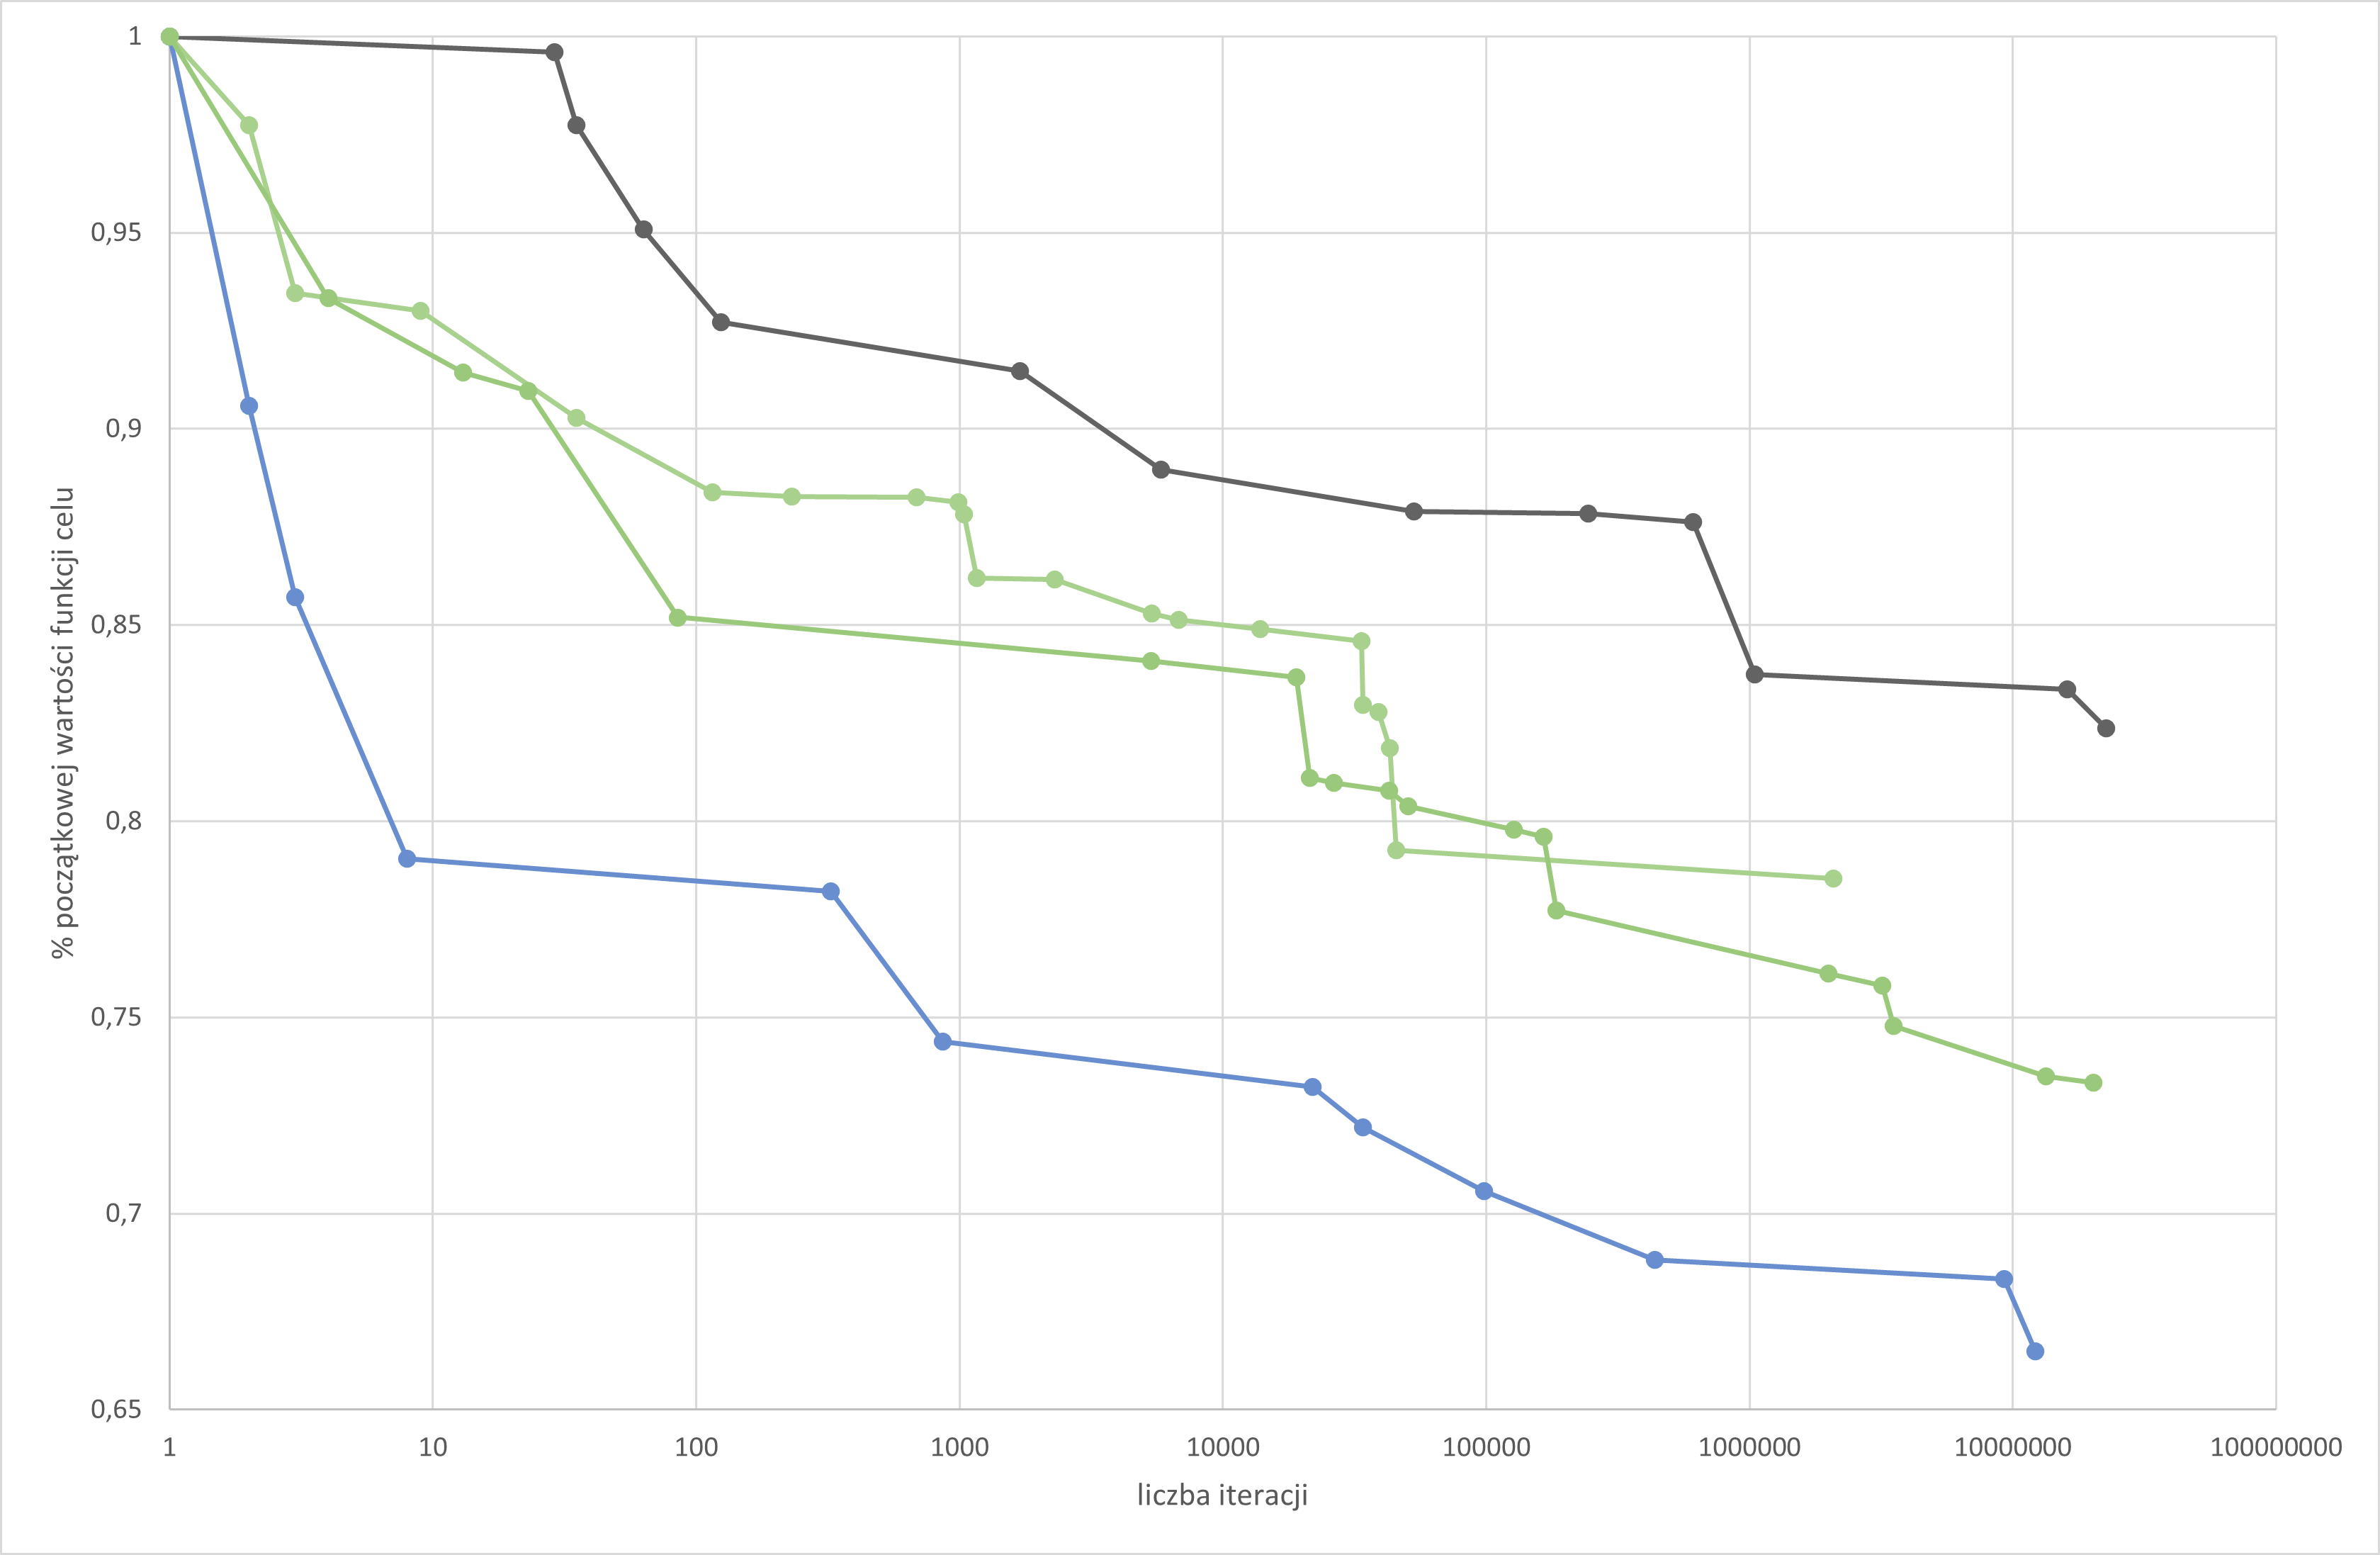
\includegraphics[scale=0.7]{k-random.png}
\caption{k-random big}
\end{figure}
Dzięki przedstawieniu wykresów w skali logarytmicznej widać, jak zachowuje się sam algorytm (w kontekście 'poprawy' rozwiązania), oraz widać jak na dłoni, że w na samym początku zazwyczaj względnie szybko znajduje nowe rozwiązania, jednak w miarę działania coraz trudniej jest wylosować rozwiązanie, które byłoby 'lepsze' od dotychczasowego najlepszego, oraz (z uwagi na jego losowość) nie jest się w stanie przewidzieć optymalnego momentu na skończenie działania (dobrze to widać dla linii 'czarne'-najwyższej, kiedy to z serii w miarę podobnych rozwiązań z małymi skokami polepszeń rzędu < 1\% - okolice 10000 do 1000000 - mamy nagle rozwiązanie lepsze o około 5\%)

\newpage
\subsubsection{Bliższe przypatrzenie się \textit{Branching Neighbor}, oraz \textit{2-Opt}}
Dodatkowo przypatrzy się jeszcze (na wykresach) co się dzieje z rozwiązaniem, kiedy podczas działania \textit{Branching} będziemy modyfikować maksymalny stopień zagłębienia (\textit{maxDepth}):
\begin{figure}[h!]
 	\centering
 	\begin{subfigure}[b]{1\linewidth}
    	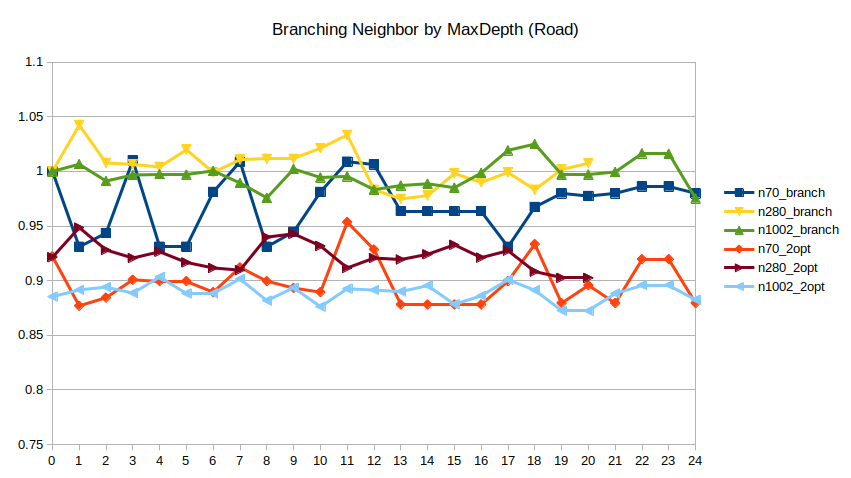
\includegraphics[width=\linewidth]{branch_roads_perc.png}
    	\caption{Porównanie procentowe względem rozwiązania bez branchingu (depth = 0)}
	\end{subfigure}
 	\begin{subfigure}[b]{1\linewidth}
    	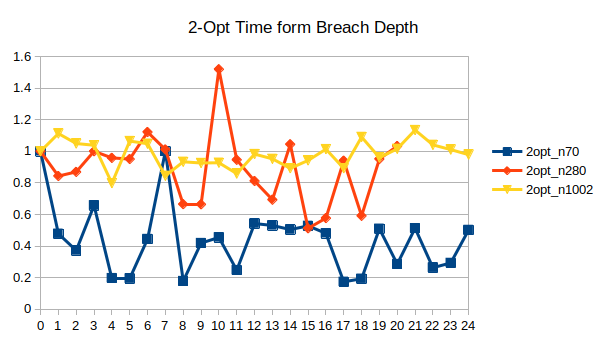
\includegraphics[width=\linewidth]{branch_times_2Opt.png}
    	\caption{czas działania dla 2-Opt'a względem rozwiązania z różną głębokością}
	\end{subfigure}
\end{figure}

\begin{figure}[h!]
 	\centering
 	\begin{subfigure}[b]{0.325\linewidth}
    	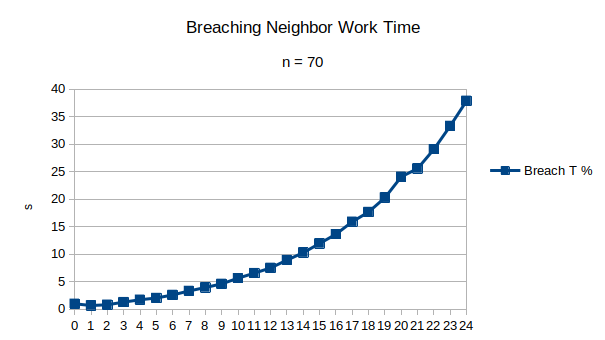
\includegraphics[width=\linewidth]{branch_times_70.png}
    	\caption{Instatncja dla n = 70}
	\end{subfigure}
	\begin{subfigure}[b]{0.325\linewidth}
    	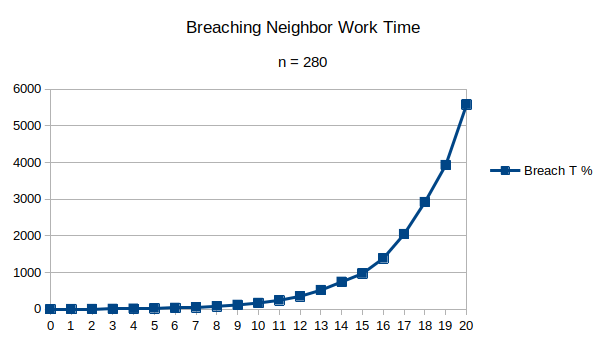
\includegraphics[width=\linewidth]{branch_times_280.png}
    	\caption{Instatncja dla n = 280}
	\end{subfigure}
	\begin{subfigure}[b]{0.325\linewidth}
    	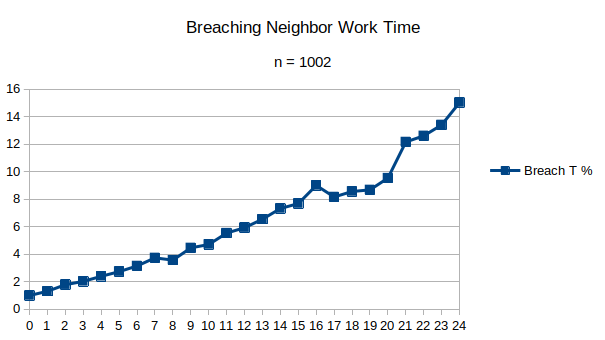
\includegraphics[width=\linewidth]{branch_times_1002.png}
    	\caption{Instatncja dla n = 1002}
	\end{subfigure}
  	\caption{Wielokrotność działania dla poszczególnych iteracji względem rozwiązania bez \textit{branchingu}}
\end{figure}

Teraz przejdźmy do analizy:
\begin{itemize}
	\item Jak widać z rysunku 3, czas działania może się drastycznie różnić w zależności od zadanego przypadku:
	\begin{itemize}
		\item a) Czas rośnie około kwadratowo
		\item b) Czas rośnie około wykładniczo
		\item c) Czas rośnie około liniowo
	\end{itemize}
	Doskonale pokazuje to, jak bardzo algorytm jest uzależniony od konkretnej instanji, jako że najbardziej 'kosztowna' operacja to właśnie 'branchowanie' w przypadku równoodległych sąsiadów, zatem jeżeli jest dużo takich przypadków (jak dla n = 280), to także czas znacznie przyśpiesza, a kiedy jest ich bardzo mało (jak dla n = 1002) to wzrost czasu jest 'względnie' niewielki
	\item Dalej w kontekście czas: Jak to widać dla wykresu czasu 2-Opta na Rysunku 1b), w zależności od przypadku jego czas działania może być dłuższy, lub krótszy, jednak cały czas będąc w przedziale $(0.2; 1.5)$ względem rozwiązania pierwotnego, zatem można zaryzykować stwierdzenie, że jego czas działania jest mało od tego zależny.
	\item Na koniec jeszcze przypatrzmy się, na wykres na rysunku 1a), gdzie widzimy porównanie funkcji celu względem rozwiązania startowego. Widzimy tutaj, że zarówno dla \textit{Branching} jak i dla \textit{2-Opt} wartości te raz skaczą 'do góry', a raz spadają 'w dół', cały czas wachając się w okolicach rzędu co najwyżej 5\%. Jakaś poprawa to jest, jednakże  w połączeniu z zestawieniami czasu, widać, że jest to mimo wszystko dosyć 'kosztowny' zysk.
\end{itemize}

\newpage
\subsubsection{Algorytmy uwspółbieżnione}

Przeprowadzono testy w celu sprawdzenia wpływu ilości rdzeni dostępnych przez algorytm k-random na czas działania algorytmu. Wartości funkcji celu dla algortymu wielowątkowego pozostały praktycznie nie zmienione (zmiany rzędu $<$ 1\%).\\
Uwspółbieżniony algorytm najbliższego sąsiada nie dał tak dobrych wyników prawdopodobnie ze względu na wadliwą implementację. Ze względów czasowych przeprowadzono testy tylko na małym przykładzie ze 100 poziomami przeszukiwań. Płytkie zagłębienie powodowało jeszcze mniejsze zyski związane z uwspółbieżnieniem.

\begin{figure}[H]
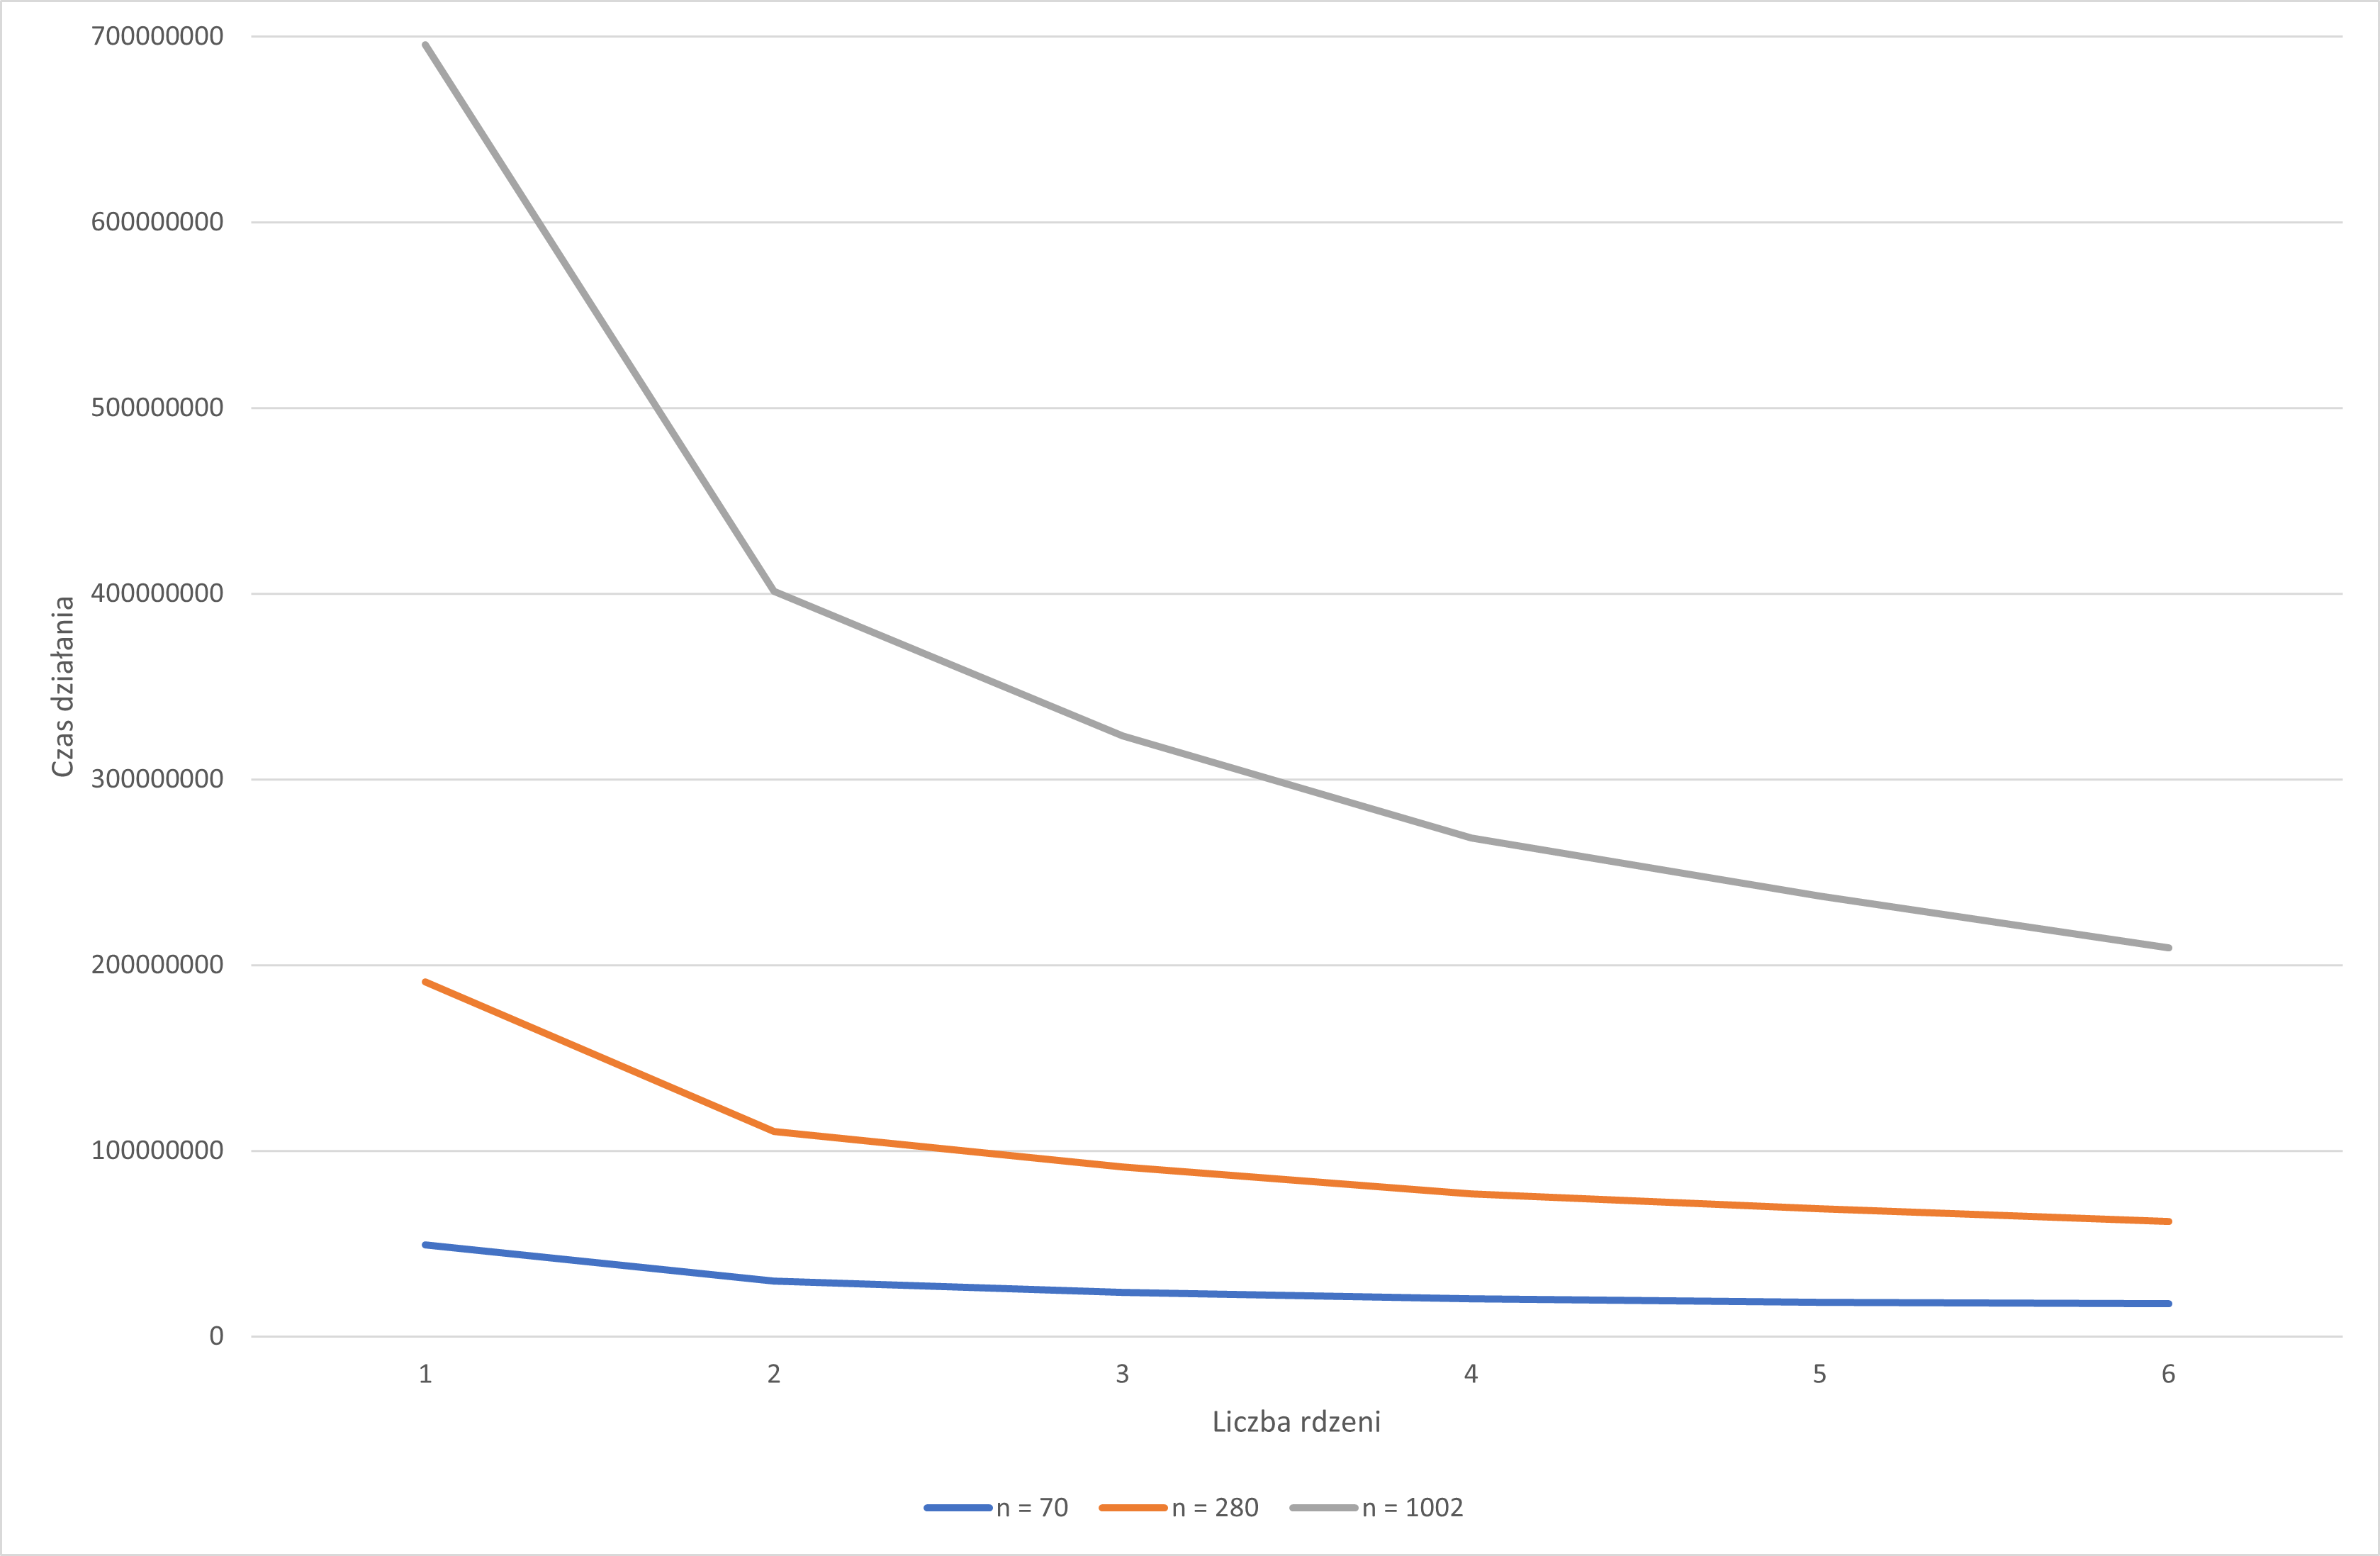
\includegraphics[scale=0.55]{k_random_parallel.png}
\caption{k-random}
\end{figure}

\begin{figure}[H]
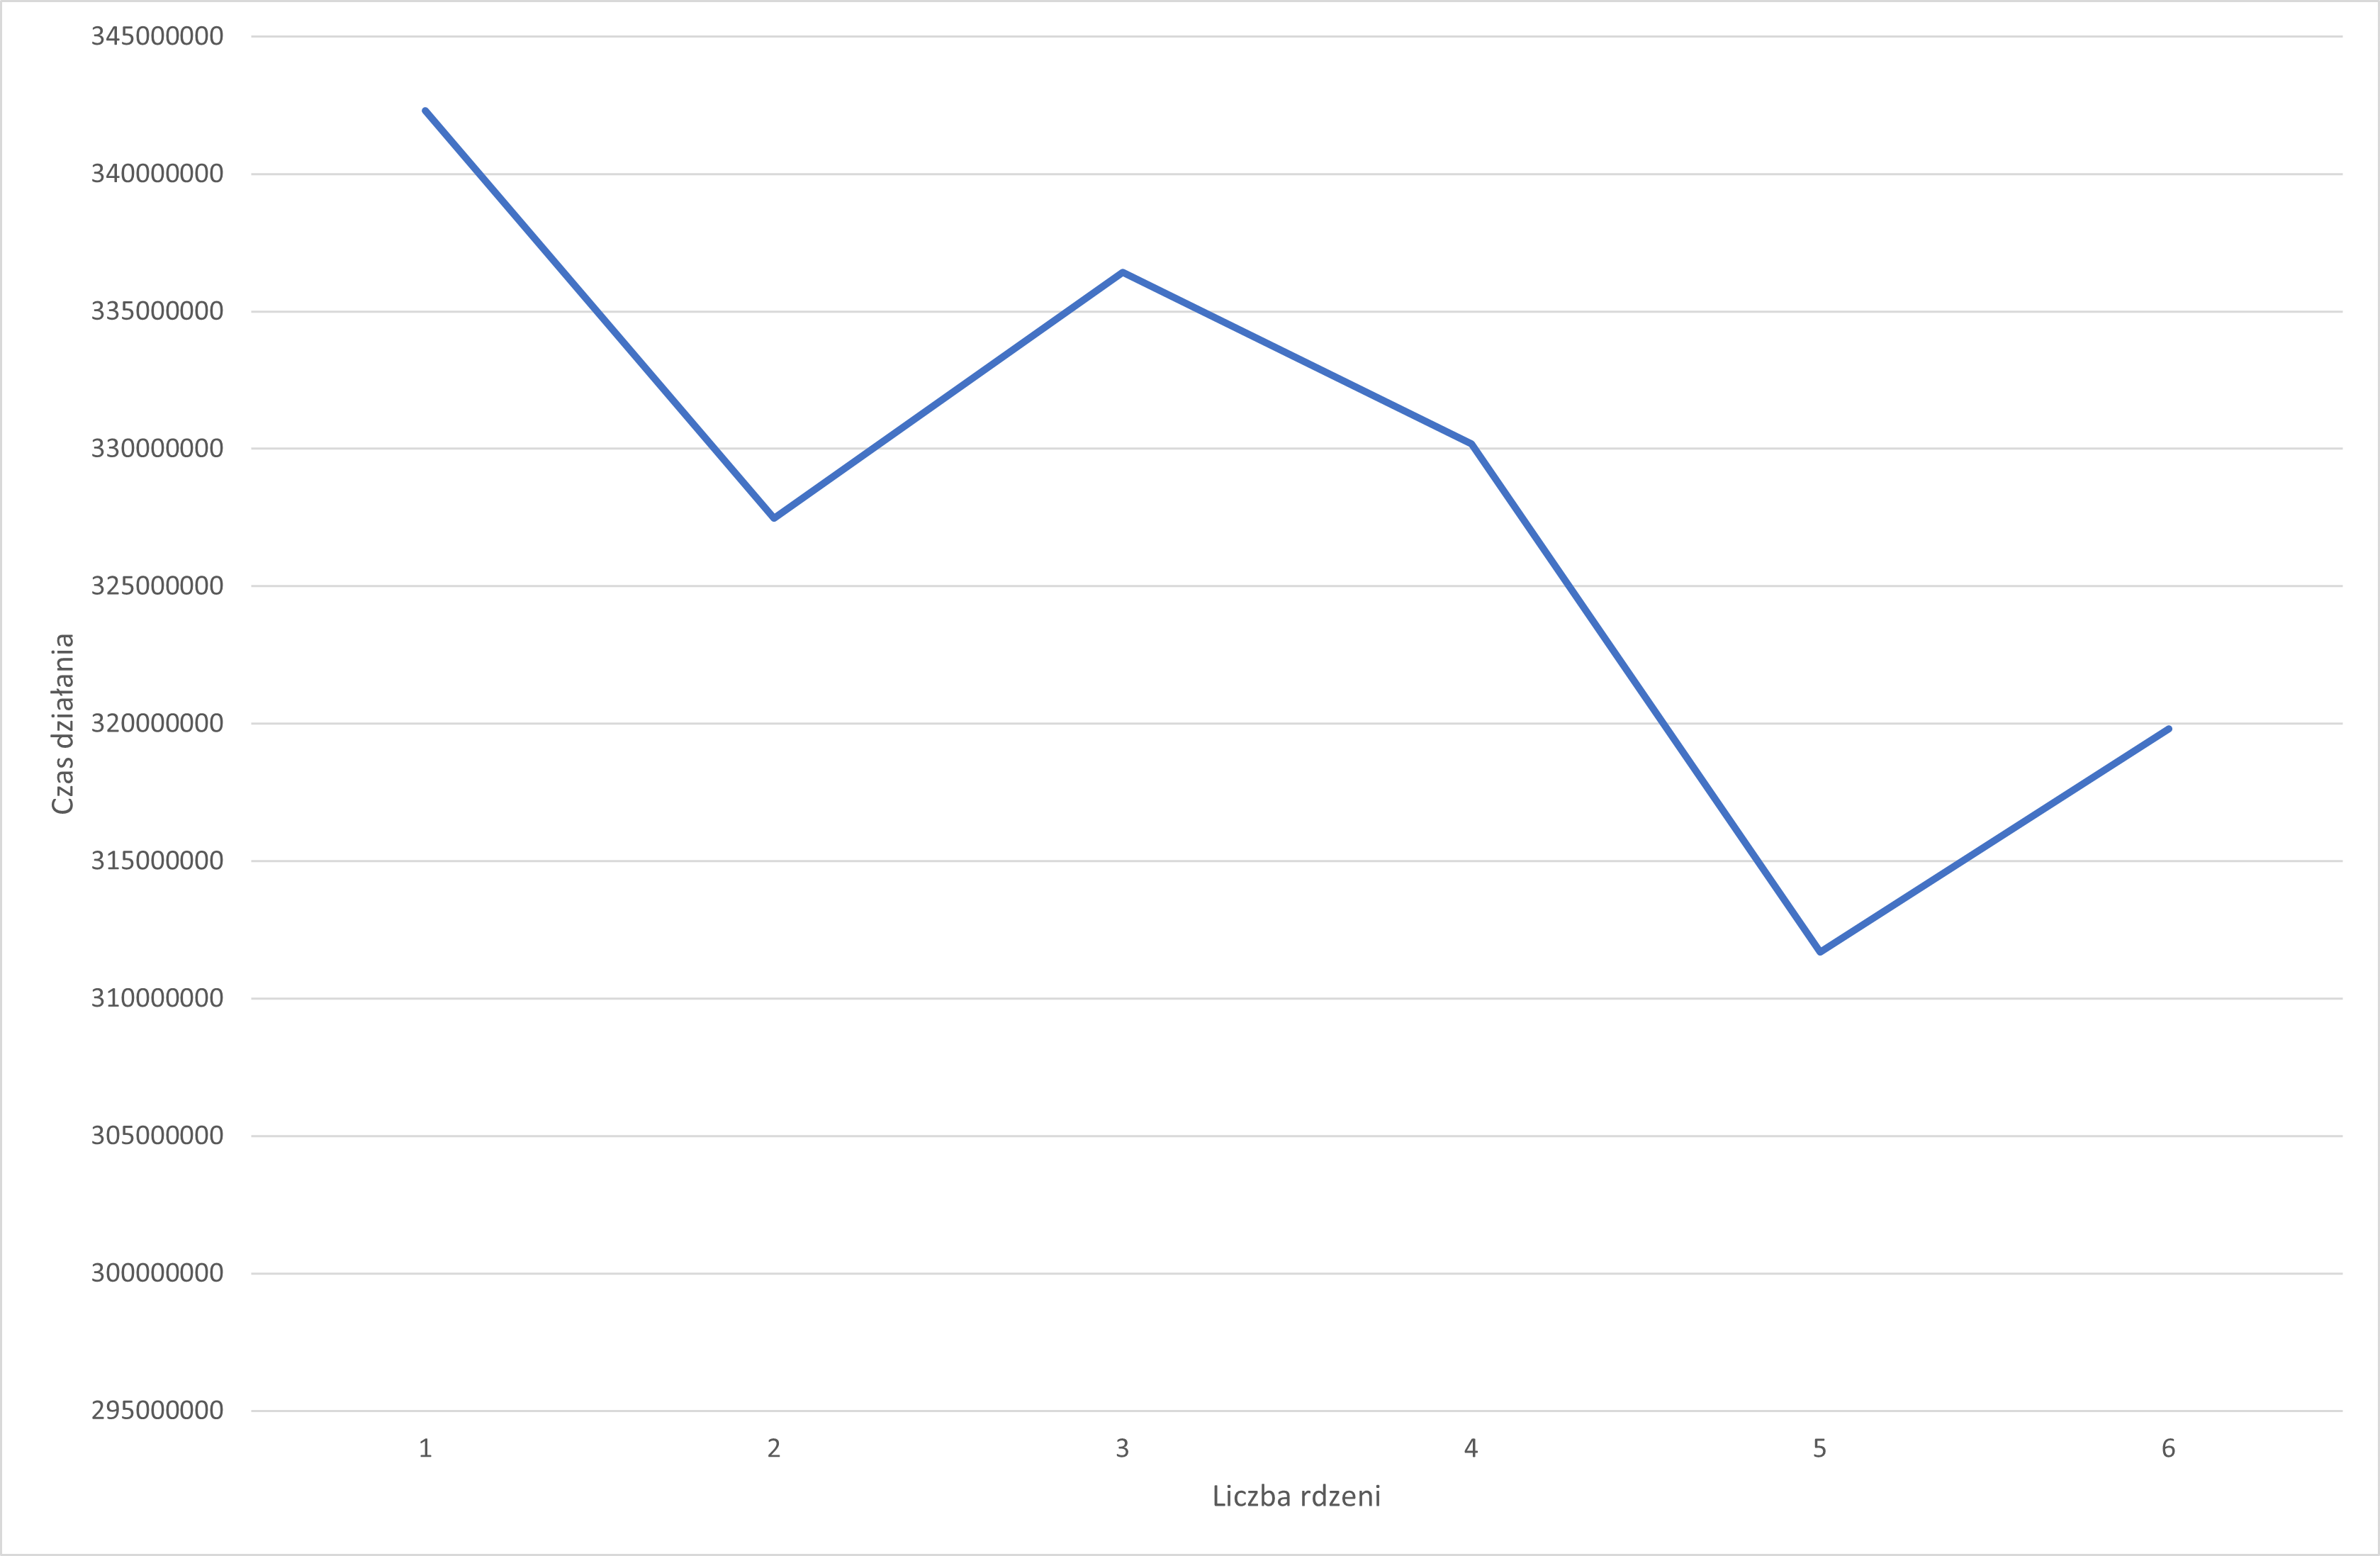
\includegraphics[scale=0.55]{nearest_neighbor_parallel.png}
\caption{Braching nearest neighbor}
\end{figure}

\subsection{Wnioski}
W większości zawarte były podczas opisu wyników, oraz przewijały się gdzieniegdzie wcześniej, jednak jednoznacznie można powiedzieć, że w znacznej większości algorytm \textit{2-Opt} okazał się zwracać najlepsze rozwiązanie w powiedzmy 'jeszcze przystępnym czasie'. 

\section*{Drobne uwagi}
Powyżej ujęte zostały 'ciekawsze' przypadki, oraz oczywiście nie opisaliśmy tutaj eksperymentów przeprowadzonch na każdej możliwej instancji z TSPLIB, ponieważ objętościowo znacznie powiększyłoby to (i tak już dosyć obszerne) sprawozdanie.\\
\\
Jako przykład takich eksperymentów, odamy tutaj wykres zrobiony dla większej liczby instancji przy testowaniu poprawy jakośći rozwiązania względem działania \textit{K-Random'a}:
\begin{figure}[H]
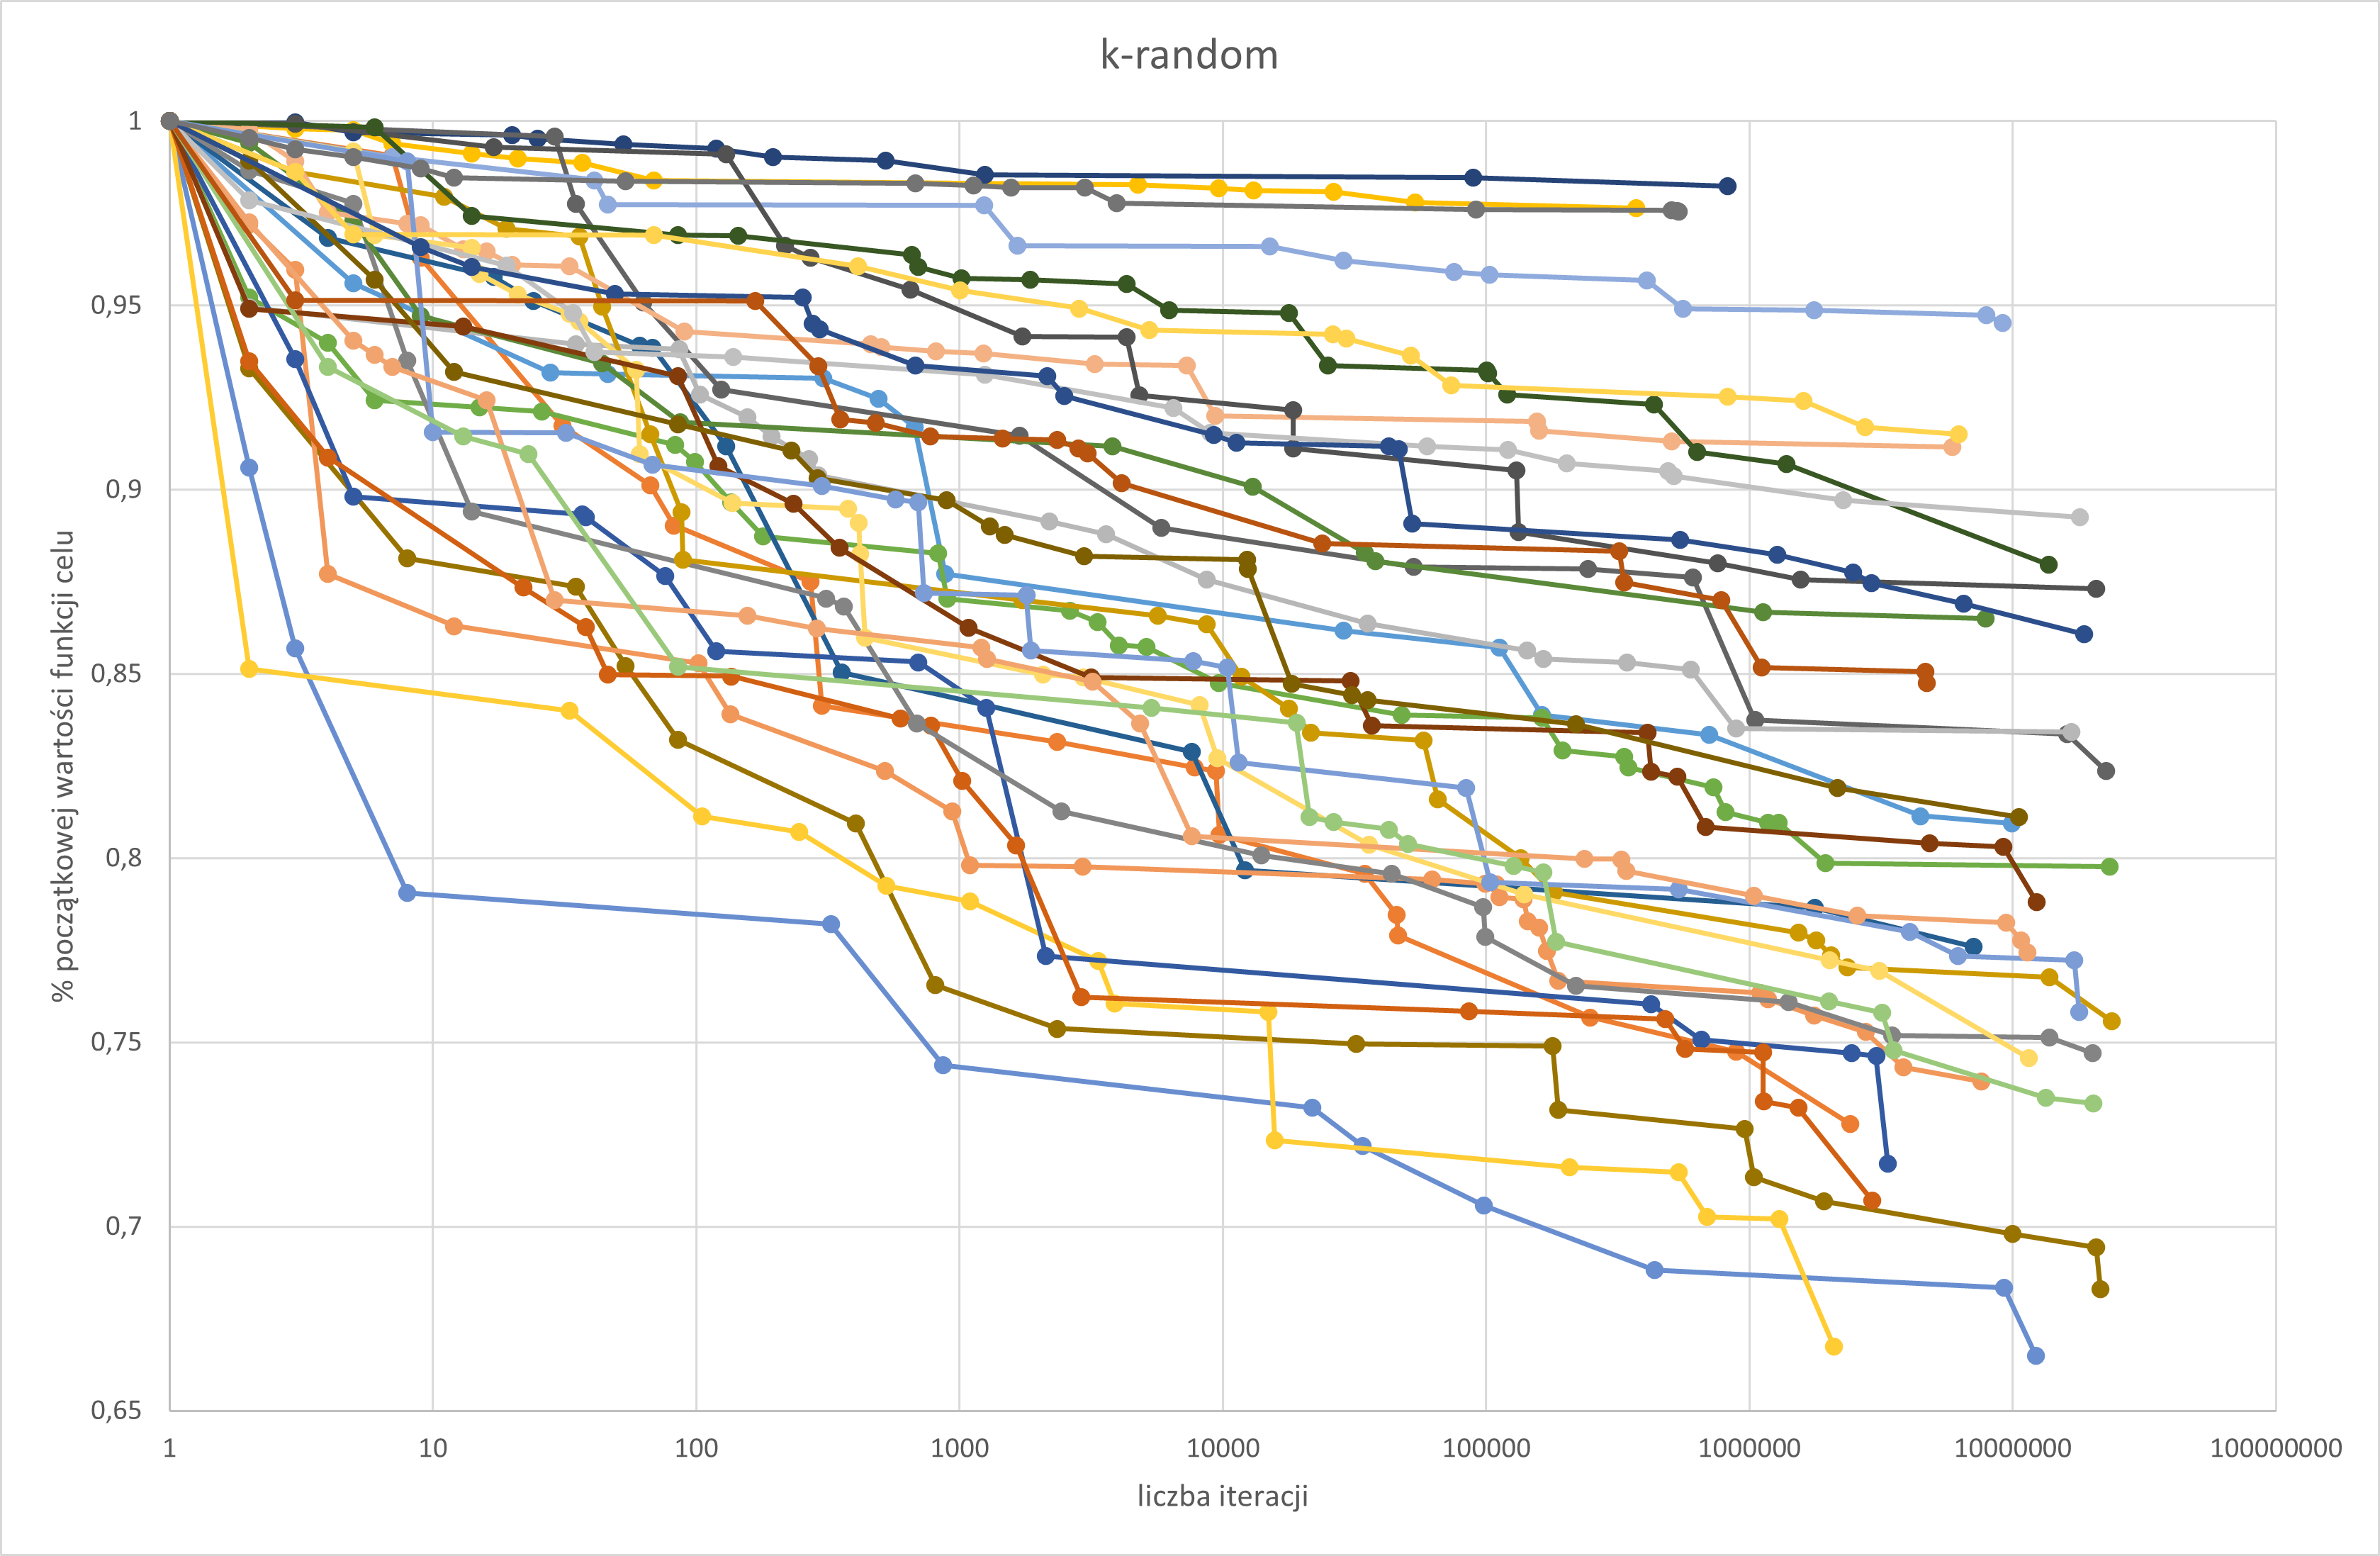
\includegraphics[scale=0.7]{k-randomFull.png}
\caption{k-random big}
\end{figure}

\end{document}